\documentclass[aspectratio=169]{beamer}
\usetheme{Bruno}
\usepackage{amsmath}
\usepackage{amssymb}
\usepackage{siunitx}
\usepackage{float}
\usepackage{tikz}
\usetikzlibrary{circuits.plc.ladder}
\usepackage{tikz-cd}
\usepackage{url}
\usepackage[siunitx,american,RPvoltages]{circuitikz}
\ctikzset{capacitors/scale=0.7}
\ctikzset{diodes/scale=0.7}
\usepackage{tabularx}
\newcolumntype{C}{>{\centering\arraybackslash}X}
\renewcommand\tabularxcolumn[1]{m{#1}}% for vertical centering text in X column
\usepackage{tabu}
\usepackage[spanish,es-tabla,activeacute]{babel}
\usepackage{babelbib}
\usepackage{booktabs}
\usepackage{pgfplots}
\usepackage{hyperref}
\hypersetup{colorlinks = true,
            linkcolor = black,
            urlcolor  = blue,
            citecolor = blue,
            anchorcolor = blue}
\usepgfplotslibrary{units, fillbetween} 
\pgfplotsset{compat=1.16}
\usepackage{bm}
\usetikzlibrary{arrows, arrows.meta, shapes, 3d, perspective, positioning}
\renewcommand{\sin}{\sen} %change from sin to sen
\usepackage{bohr}
\setbohr{distribution-method = quantum,insert-missing = true}
\usepackage{elements}
\usepackage{verbatim}
\usetikzlibrary{mindmap,trees,backgrounds}
\definecolor{color_mate}{RGB}{255,255,128}
\definecolor{color_plas}{RGB}{255,128,255}
\definecolor{color_text}{RGB}{128,255,255}
\definecolor{color_petr}{RGB}{255,192,192}
\definecolor{color_made}{RGB}{192,255,192}
\definecolor{color_meta}{RGB}{192,192,255}
\usepackage[edges]{forest}
\usepackage{etoolbox}
\usepackage{schemata}
\newcommand\diagram[2]{\schema{\schemabox{#1}}{\schemabox{#2}}}
\usepackage{listings}
\usepackage{csvsimple}
 %%%%%%%%%%%%%%%%%%%%%%%%%%%%%%%%%%%%%%%%%%%%%%%%%%%%%%%%%%%%%%%%%%%%%%%%%%%%%%%% 
%%% ~ Arduino Language - Arduino IDE Colors ~                                  %%%
%%%                                                                            %%%
%%% Kyle Rocha-Brownell | 10/2/2017 | No Licence                               %%%
%%% -------------------------------------------------------------------------- %%%
%%%                                                                            %%%
%%% Place this file in your working directory (next to the latex file you're   %%%
%%% working on).  To add it to your project, place:                            %%%
%%%     %%%%%%%%%%%%%%%%%%%%%%%%%%%%%%%%%%%%%%%%%%%%%%%%%%%%%%%%%%%%%%%%%%%%%%%%%%%%%%%% 
%%% ~ Arduino Language - Arduino IDE Colors ~                                  %%%
%%%                                                                            %%%
%%% Kyle Rocha-Brownell | 10/2/2017 | No Licence                               %%%
%%% -------------------------------------------------------------------------- %%%
%%%                                                                            %%%
%%% Place this file in your working directory (next to the latex file you're   %%%
%%% working on).  To add it to your project, place:                            %%%
%%%    \input{arduinoLanguage.tex}                                             %%%
%%% somewhere before \begin{document} in your latex file.                      %%%
%%%                                                                            %%%
%%% In your document, place your arduino code between:                         %%%
%%%   \begin{lstlisting}[language=Arduino]                                     %%%
%%% and:                                                                       %%%
%%%   \end{lstlisting}                                                         %%%
%%%                                                                            %%%
%%% Or create your own style to add non-built-in functions and variables.      %%%
%%%                                                                            %%%
 %%%%%%%%%%%%%%%%%%%%%%%%%%%%%%%%%%%%%%%%%%%%%%%%%%%%%%%%%%%%%%%%%%%%%%%%%%%%%%%% 

\usepackage{color}
\usepackage{listings}    
\usepackage{courier}

%%% Define Custom IDE Colors %%%
\definecolor{arduinoGreen}    {rgb} {0.17, 0.43, 0.01}
\definecolor{arduinoGrey}     {rgb} {0.47, 0.47, 0.33}
\definecolor{arduinoOrange}   {rgb} {0.8 , 0.4 , 0   }
\definecolor{arduinoBlue}     {rgb} {0.01, 0.61, 0.98}
\definecolor{arduinoDarkBlue} {rgb} {0.0 , 0.2 , 0.5 }

%%% Define Arduino Language %%%
\lstdefinelanguage{Arduino}{
  language=C++, % begin with default C++ settings 
%
%
  %%% Keyword Color Group 1 %%%  (called KEYWORD3 by arduino)
  keywordstyle=\color{arduinoGreen},   
  deletekeywords={  % remove all arduino keywords that might be in c++
                break, case, override, final, continue, default, do, else, for, 
                if, return, goto, switch, throw, try, while, setup, loop, export, 
                not, or, and, xor, include, define, elif, else, error, if, ifdef, 
                ifndef, pragma, warning,
                HIGH, LOW, INPUT, INPUT_PULLUP, OUTPUT, DEC, BIN, HEX, OCT, PI, 
                HALF_PI, TWO_PI, LSBFIRST, MSBFIRST, CHANGE, FALLING, RISING, 
                DEFAULT, EXTERNAL, INTERNAL, INTERNAL1V1, INTERNAL2V56, LED_BUILTIN, 
                LED_BUILTIN_RX, LED_BUILTIN_TX, DIGITAL_MESSAGE, FIRMATA_STRING, 
                ANALOG_MESSAGE, REPORT_DIGITAL, REPORT_ANALOG, SET_PIN_MODE, 
                SYSTEM_RESET, SYSEX_START, auto, int8_t, int16_t, int32_t, int64_t, 
                uint8_t, uint16_t, uint32_t, uint64_t, char16_t, char32_t, operator, 
                enum, delete, bool, boolean, byte, char, const, false, float, double, 
                null, NULL, int, long, new, private, protected, public, short, 
                signed, static, volatile, String, void, true, unsigned, word, array, 
                sizeof, dynamic_cast, typedef, const_cast, struct, static_cast, union, 
                friend, extern, class, reinterpret_cast, register, explicit, inline, 
                _Bool, complex, _Complex, _Imaginary, atomic_bool, atomic_char, 
                atomic_schar, atomic_uchar, atomic_short, atomic_ushort, atomic_int, 
                atomic_uint, atomic_long, atomic_ulong, atomic_llong, atomic_ullong, 
                virtual, PROGMEM,
                Serial, Serial1, Serial2, Serial3, SerialUSB, Keyboard, Mouse,
                abs, acos, asin, atan, atan2, ceil, constrain, cos, degrees, exp, 
                floor, log, map, max, min, radians, random, randomSeed, round, sin, 
                sq, sqrt, tan, pow, bitRead, bitWrite, bitSet, bitClear, bit, 
                highByte, lowByte, analogReference, analogRead, 
                analogReadResolution, analogWrite, analogWriteResolution, 
                attachInterrupt, detachInterrupt, digitalPinToInterrupt, delay, 
                delayMicroseconds, digitalWrite, digitalRead, interrupts, millis, 
                micros, noInterrupts, noTone, pinMode, pulseIn, pulseInLong, shiftIn, 
                shiftOut, tone, yield, Stream, begin, end, peek, read, print, 
                println, available, availableForWrite, flush, setTimeout, find, 
                findUntil, parseInt, parseFloat, readBytes, readBytesUntil, readString, 
                readStringUntil, trim, toUpperCase, toLowerCase, charAt, compareTo, 
                concat, endsWith, startsWith, equals, equalsIgnoreCase, getBytes, 
                indexOf, lastIndexOf, length, replace, setCharAt, substring, 
                toCharArray, toInt, press, release, releaseAll, accept, click, move, 
                isPressed, isAlphaNumeric, isAlpha, isAscii, isWhitespace, isControl, 
                isDigit, isGraph, isLowerCase, isPrintable, isPunct, isSpace, 
                isUpperCase, isHexadecimalDigit, 
                }, 
  morekeywords={   % add arduino structures to group 1
                break, case, override, final, continue, default, do, else, for, 
                if, return, goto, switch, throw, try, while, setup, loop, export, 
                not, or, and, xor, include, define, elif, else, error, if, ifdef, 
                ifndef, pragma, warning,
                }, 
% 
%
  %%% Keyword Color Group 2 %%%  (called LITERAL1 by arduino)
  keywordstyle=[2]\color{arduinoBlue},   
  keywords=[2]{   % add variables and dataTypes as 2nd group  
                HIGH, LOW, INPUT, INPUT_PULLUP, OUTPUT, DEC, BIN, HEX, OCT, PI, 
                HALF_PI, TWO_PI, LSBFIRST, MSBFIRST, CHANGE, FALLING, RISING, 
                DEFAULT, EXTERNAL, INTERNAL, INTERNAL1V1, INTERNAL2V56, LED_BUILTIN, 
                LED_BUILTIN_RX, LED_BUILTIN_TX, DIGITAL_MESSAGE, FIRMATA_STRING, 
                ANALOG_MESSAGE, REPORT_DIGITAL, REPORT_ANALOG, SET_PIN_MODE, 
                SYSTEM_RESET, SYSEX_START, auto, int8_t, int16_t, int32_t, int64_t, 
                uint8_t, uint16_t, uint32_t, uint64_t, char16_t, char32_t, operator, 
                enum, delete, bool, boolean, byte, char, const, false, float, double, 
                null, NULL, int, long, new, private, protected, public, short, 
                signed, static, volatile, String, void, true, unsigned, word, array, 
                sizeof, dynamic_cast, typedef, const_cast, struct, static_cast, union, 
                friend, extern, class, reinterpret_cast, register, explicit, inline, 
                _Bool, complex, _Complex, _Imaginary, atomic_bool, atomic_char, 
                atomic_schar, atomic_uchar, atomic_short, atomic_ushort, atomic_int, 
                atomic_uint, atomic_long, atomic_ulong, atomic_llong, atomic_ullong, 
                virtual, PROGMEM,
                },  
% 
%
  %%% Keyword Color Group 3 %%%  (called KEYWORD1 by arduino)
  keywordstyle=[3]\bfseries\color{arduinoOrange},
  keywords=[3]{  % add built-in functions as a 3rd group
                Serial, Serial1, Serial2, Serial3, SerialUSB, Keyboard, Mouse,
                },      
%
%
  %%% Keyword Color Group 4 %%%  (called KEYWORD2 by arduino)
  keywordstyle=[4]\color{arduinoOrange},
  keywords=[4]{  % add more built-in functions as a 4th group
                abs, acos, asin, atan, atan2, ceil, constrain, cos, degrees, exp, 
                floor, log, map, max, min, radians, random, randomSeed, round, sin, 
                sq, sqrt, tan, pow, bitRead, bitWrite, bitSet, bitClear, bit, 
                highByte, lowByte, analogReference, analogRead, 
                analogReadResolution, analogWrite, analogWriteResolution, 
                attachInterrupt, detachInterrupt, digitalPinToInterrupt, delay, 
                delayMicroseconds, digitalWrite, digitalRead, interrupts, millis, 
                micros, noInterrupts, noTone, pinMode, pulseIn, pulseInLong, shiftIn, 
                shiftOut, tone, yield, Stream, begin, end, peek, read, print, 
                println, available, availableForWrite, flush, setTimeout, find, 
                findUntil, parseInt, parseFloat, readBytes, readBytesUntil, readString, 
                readStringUntil, trim, toUpperCase, toLowerCase, charAt, compareTo, 
                concat, endsWith, startsWith, equals, equalsIgnoreCase, getBytes, 
                indexOf, lastIndexOf, length, replace, setCharAt, substring, 
                toCharArray, toInt, press, release, releaseAll, accept, click, move, 
                isPressed, isAlphaNumeric, isAlpha, isAscii, isWhitespace, isControl, 
                isDigit, isGraph, isLowerCase, isPrintable, isPunct, isSpace, 
                isUpperCase, isHexadecimalDigit, 
                },      
%
%
  %%% Set Other Colors %%%
  stringstyle=\color{arduinoDarkBlue},    
  commentstyle=\color{arduinoGrey},    
%          
%   
  %%%% Line Numbering %%%%
   numbers=left,                    
  numbersep=5pt,                   
  numberstyle=\color{arduinoGrey},    
  %stepnumber=2,                      % show every 2 line numbers
%
%
  %%%% Code Box Style %%%%
  breaklines=true,                    % wordwrapping
  tabsize=2,         
  basicstyle=\ttfamily  
}                                             %%%
%%% somewhere before \begin{document} in your latex file.                      %%%
%%%                                                                            %%%
%%% In your document, place your arduino code between:                         %%%
%%%   \begin{lstlisting}[language=Arduino]                                     %%%
%%% and:                                                                       %%%
%%%   \end{lstlisting}                                                         %%%
%%%                                                                            %%%
%%% Or create your own style to add non-built-in functions and variables.      %%%
%%%                                                                            %%%
 %%%%%%%%%%%%%%%%%%%%%%%%%%%%%%%%%%%%%%%%%%%%%%%%%%%%%%%%%%%%%%%%%%%%%%%%%%%%%%%% 

\usepackage{color}
\usepackage{listings}    
\usepackage{courier}

%%% Define Custom IDE Colors %%%
\definecolor{arduinoGreen}    {rgb} {0.17, 0.43, 0.01}
\definecolor{arduinoGrey}     {rgb} {0.47, 0.47, 0.33}
\definecolor{arduinoOrange}   {rgb} {0.8 , 0.4 , 0   }
\definecolor{arduinoBlue}     {rgb} {0.01, 0.61, 0.98}
\definecolor{arduinoDarkBlue} {rgb} {0.0 , 0.2 , 0.5 }

%%% Define Arduino Language %%%
\lstdefinelanguage{Arduino}{
  language=C++, % begin with default C++ settings 
%
%
  %%% Keyword Color Group 1 %%%  (called KEYWORD3 by arduino)
  keywordstyle=\color{arduinoGreen},   
  deletekeywords={  % remove all arduino keywords that might be in c++
                break, case, override, final, continue, default, do, else, for, 
                if, return, goto, switch, throw, try, while, setup, loop, export, 
                not, or, and, xor, include, define, elif, else, error, if, ifdef, 
                ifndef, pragma, warning,
                HIGH, LOW, INPUT, INPUT_PULLUP, OUTPUT, DEC, BIN, HEX, OCT, PI, 
                HALF_PI, TWO_PI, LSBFIRST, MSBFIRST, CHANGE, FALLING, RISING, 
                DEFAULT, EXTERNAL, INTERNAL, INTERNAL1V1, INTERNAL2V56, LED_BUILTIN, 
                LED_BUILTIN_RX, LED_BUILTIN_TX, DIGITAL_MESSAGE, FIRMATA_STRING, 
                ANALOG_MESSAGE, REPORT_DIGITAL, REPORT_ANALOG, SET_PIN_MODE, 
                SYSTEM_RESET, SYSEX_START, auto, int8_t, int16_t, int32_t, int64_t, 
                uint8_t, uint16_t, uint32_t, uint64_t, char16_t, char32_t, operator, 
                enum, delete, bool, boolean, byte, char, const, false, float, double, 
                null, NULL, int, long, new, private, protected, public, short, 
                signed, static, volatile, String, void, true, unsigned, word, array, 
                sizeof, dynamic_cast, typedef, const_cast, struct, static_cast, union, 
                friend, extern, class, reinterpret_cast, register, explicit, inline, 
                _Bool, complex, _Complex, _Imaginary, atomic_bool, atomic_char, 
                atomic_schar, atomic_uchar, atomic_short, atomic_ushort, atomic_int, 
                atomic_uint, atomic_long, atomic_ulong, atomic_llong, atomic_ullong, 
                virtual, PROGMEM,
                Serial, Serial1, Serial2, Serial3, SerialUSB, Keyboard, Mouse,
                abs, acos, asin, atan, atan2, ceil, constrain, cos, degrees, exp, 
                floor, log, map, max, min, radians, random, randomSeed, round, sin, 
                sq, sqrt, tan, pow, bitRead, bitWrite, bitSet, bitClear, bit, 
                highByte, lowByte, analogReference, analogRead, 
                analogReadResolution, analogWrite, analogWriteResolution, 
                attachInterrupt, detachInterrupt, digitalPinToInterrupt, delay, 
                delayMicroseconds, digitalWrite, digitalRead, interrupts, millis, 
                micros, noInterrupts, noTone, pinMode, pulseIn, pulseInLong, shiftIn, 
                shiftOut, tone, yield, Stream, begin, end, peek, read, print, 
                println, available, availableForWrite, flush, setTimeout, find, 
                findUntil, parseInt, parseFloat, readBytes, readBytesUntil, readString, 
                readStringUntil, trim, toUpperCase, toLowerCase, charAt, compareTo, 
                concat, endsWith, startsWith, equals, equalsIgnoreCase, getBytes, 
                indexOf, lastIndexOf, length, replace, setCharAt, substring, 
                toCharArray, toInt, press, release, releaseAll, accept, click, move, 
                isPressed, isAlphaNumeric, isAlpha, isAscii, isWhitespace, isControl, 
                isDigit, isGraph, isLowerCase, isPrintable, isPunct, isSpace, 
                isUpperCase, isHexadecimalDigit, 
                }, 
  morekeywords={   % add arduino structures to group 1
                break, case, override, final, continue, default, do, else, for, 
                if, return, goto, switch, throw, try, while, setup, loop, export, 
                not, or, and, xor, include, define, elif, else, error, if, ifdef, 
                ifndef, pragma, warning,
                }, 
% 
%
  %%% Keyword Color Group 2 %%%  (called LITERAL1 by arduino)
  keywordstyle=[2]\color{arduinoBlue},   
  keywords=[2]{   % add variables and dataTypes as 2nd group  
                HIGH, LOW, INPUT, INPUT_PULLUP, OUTPUT, DEC, BIN, HEX, OCT, PI, 
                HALF_PI, TWO_PI, LSBFIRST, MSBFIRST, CHANGE, FALLING, RISING, 
                DEFAULT, EXTERNAL, INTERNAL, INTERNAL1V1, INTERNAL2V56, LED_BUILTIN, 
                LED_BUILTIN_RX, LED_BUILTIN_TX, DIGITAL_MESSAGE, FIRMATA_STRING, 
                ANALOG_MESSAGE, REPORT_DIGITAL, REPORT_ANALOG, SET_PIN_MODE, 
                SYSTEM_RESET, SYSEX_START, auto, int8_t, int16_t, int32_t, int64_t, 
                uint8_t, uint16_t, uint32_t, uint64_t, char16_t, char32_t, operator, 
                enum, delete, bool, boolean, byte, char, const, false, float, double, 
                null, NULL, int, long, new, private, protected, public, short, 
                signed, static, volatile, String, void, true, unsigned, word, array, 
                sizeof, dynamic_cast, typedef, const_cast, struct, static_cast, union, 
                friend, extern, class, reinterpret_cast, register, explicit, inline, 
                _Bool, complex, _Complex, _Imaginary, atomic_bool, atomic_char, 
                atomic_schar, atomic_uchar, atomic_short, atomic_ushort, atomic_int, 
                atomic_uint, atomic_long, atomic_ulong, atomic_llong, atomic_ullong, 
                virtual, PROGMEM,
                },  
% 
%
  %%% Keyword Color Group 3 %%%  (called KEYWORD1 by arduino)
  keywordstyle=[3]\bfseries\color{arduinoOrange},
  keywords=[3]{  % add built-in functions as a 3rd group
                Serial, Serial1, Serial2, Serial3, SerialUSB, Keyboard, Mouse,
                },      
%
%
  %%% Keyword Color Group 4 %%%  (called KEYWORD2 by arduino)
  keywordstyle=[4]\color{arduinoOrange},
  keywords=[4]{  % add more built-in functions as a 4th group
                abs, acos, asin, atan, atan2, ceil, constrain, cos, degrees, exp, 
                floor, log, map, max, min, radians, random, randomSeed, round, sin, 
                sq, sqrt, tan, pow, bitRead, bitWrite, bitSet, bitClear, bit, 
                highByte, lowByte, analogReference, analogRead, 
                analogReadResolution, analogWrite, analogWriteResolution, 
                attachInterrupt, detachInterrupt, digitalPinToInterrupt, delay, 
                delayMicroseconds, digitalWrite, digitalRead, interrupts, millis, 
                micros, noInterrupts, noTone, pinMode, pulseIn, pulseInLong, shiftIn, 
                shiftOut, tone, yield, Stream, begin, end, peek, read, print, 
                println, available, availableForWrite, flush, setTimeout, find, 
                findUntil, parseInt, parseFloat, readBytes, readBytesUntil, readString, 
                readStringUntil, trim, toUpperCase, toLowerCase, charAt, compareTo, 
                concat, endsWith, startsWith, equals, equalsIgnoreCase, getBytes, 
                indexOf, lastIndexOf, length, replace, setCharAt, substring, 
                toCharArray, toInt, press, release, releaseAll, accept, click, move, 
                isPressed, isAlphaNumeric, isAlpha, isAscii, isWhitespace, isControl, 
                isDigit, isGraph, isLowerCase, isPrintable, isPunct, isSpace, 
                isUpperCase, isHexadecimalDigit, 
                },      
%
%
  %%% Set Other Colors %%%
  stringstyle=\color{arduinoDarkBlue},    
  commentstyle=\color{arduinoGrey},    
%          
%   
  %%%% Line Numbering %%%%
   numbers=left,                    
  numbersep=5pt,                   
  numberstyle=\color{arduinoGrey},    
  %stepnumber=2,                      % show every 2 line numbers
%
%
  %%%% Code Box Style %%%%
  breaklines=true,                    % wordwrapping
  tabsize=2,         
  basicstyle=\ttfamily  
}
\usepackage{lmodern}
\usepackage{subcaption}

\graphicspath{{../fig/}}


\title{Lab Control Eléctrico: \\ \emph{Introducción a Arduino}}
\author{
    Juan J. Rojas
}
\institute{Instituto Tecnológico de Costa Rica}
\date{\today}
\background{fig/background.jpg}
\begin{document}
%\sisetup{unit-math-rm=\mathrm,math-rm=\mathrm} % change sinitx font
\sisetup{output-decimal-marker = {,}}
\maketitle

\newcommand{\blackandwhite}{white} %change this at the end


\begin{frame}[t]{Sistemas embebidos}
Es un computador diseñado para realizar alguna función específica dentro de un sistema complejo. Típicamente opera sin intervención del usuario a diferencia de un computador personal.  

\begin{tikzpicture}[remember picture, overlay]
    \node[above=0.5cm] at (current page.south) 
    {
        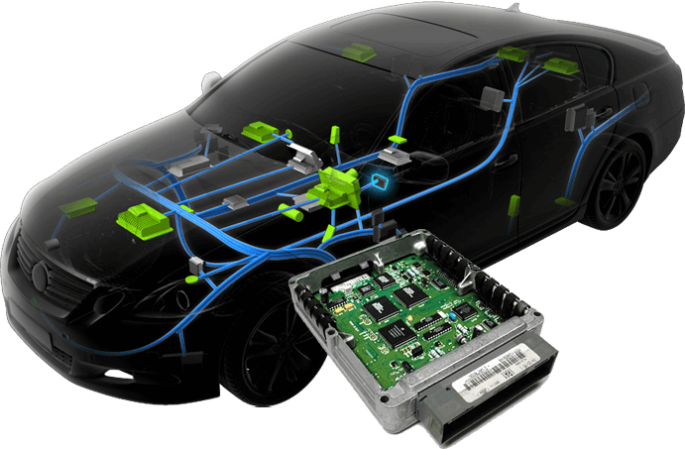
\includegraphics[width=0.55\textwidth]{fig/embebidos.png}
    };
\end{tikzpicture}
\end{frame}

\begin{frame}[t]{Microcontroladores}
Son circuitos integrados compactos diseñados para gobernar alguna operación específica en un sistema embebido. Incluyen un procesador, memoria (RAM y ROM/flash) y periféricos de entrada/salida en un solo chip.

\begin{tikzpicture}[remember picture, overlay]
    \node[above=0.5cm] at (current page.south) 
    {
        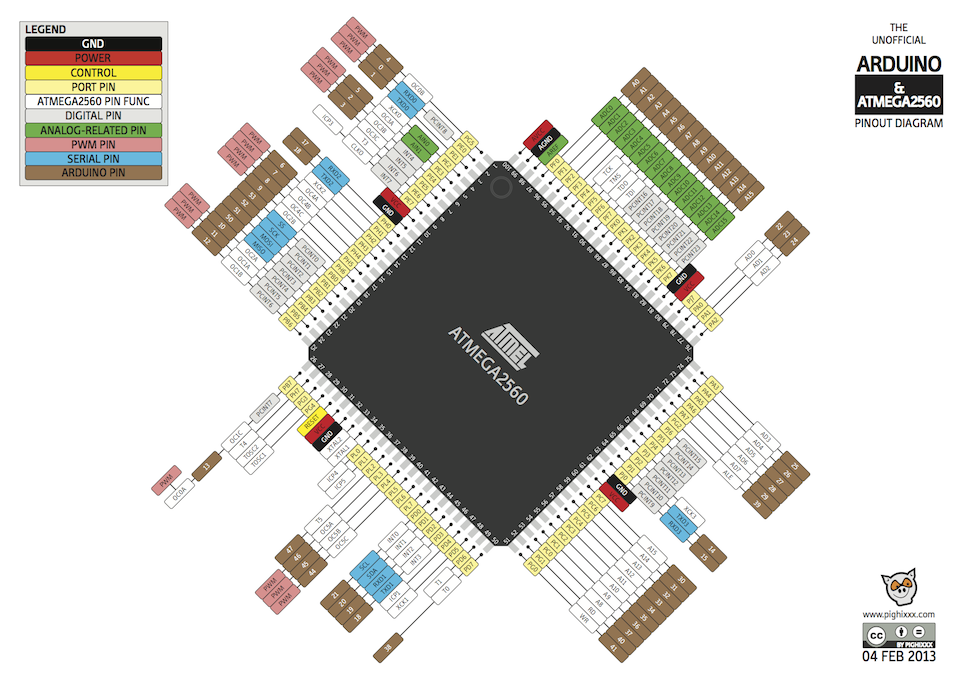
\includegraphics[width=0.5\textwidth]{fig/ATMEGA2560.png}
    };
\end{tikzpicture}
\end{frame}

\begin{frame}[t]{Placas de desarrollo}
Son plataformas de hardware diseñadas para ayudar a crear y validar aplicaciones de sistemas embebidos. Estas placas generalmente incluyen un microcontrolador o microprocesador, junto con una serie de periféricos y conectores que facilitan la conexión de sensores, actuadores, y otros componentes necesarios para el desarrollo de un proyecto embebido.

\begin{tikzpicture}[remember picture, overlay]
    \node[above=0.5cm] at (current page.south) 
    {
        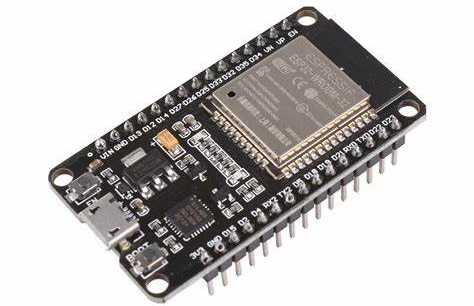
\includegraphics[width=0.5\textwidth]{fig/ESP32.jpeg}
    };
\end{tikzpicture}
\end{frame}



\begin{frame}[t]{Lenguajes de programación: niveles}
El nivel de un lenguaje de programación se define según su relación con el lenguaje humano. Un lenguaje de programación de alto nivel es uno que está mas cerca de los lenguajes humanos y mas lejos del lenguaje de máquina

\begin{tikzpicture}[remember picture, overlay]
    \node[above] at (current page.south) 
    {
        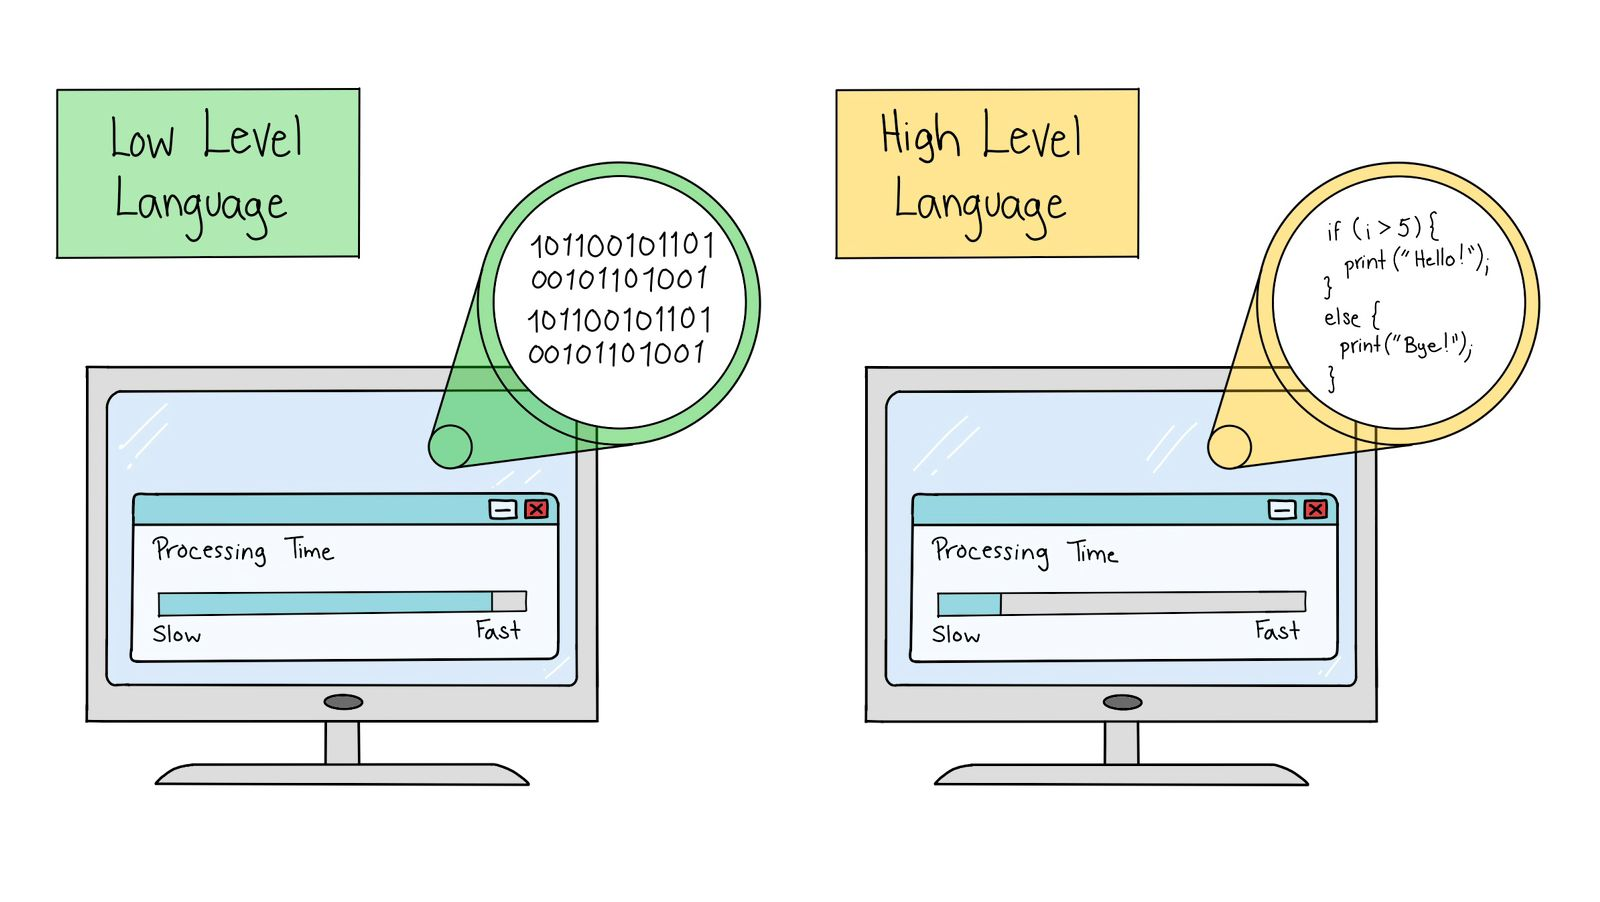
\includegraphics[width=0.7\textwidth]{fig/niveles.jpg}
    };
\end{tikzpicture}
\end{frame}

\begin{frame}[t]{Lenguajes de programación: compilado o interpretado}

\begin{tikzpicture}[remember picture, overlay]
    \node[above] at (current page.south) 
    {
        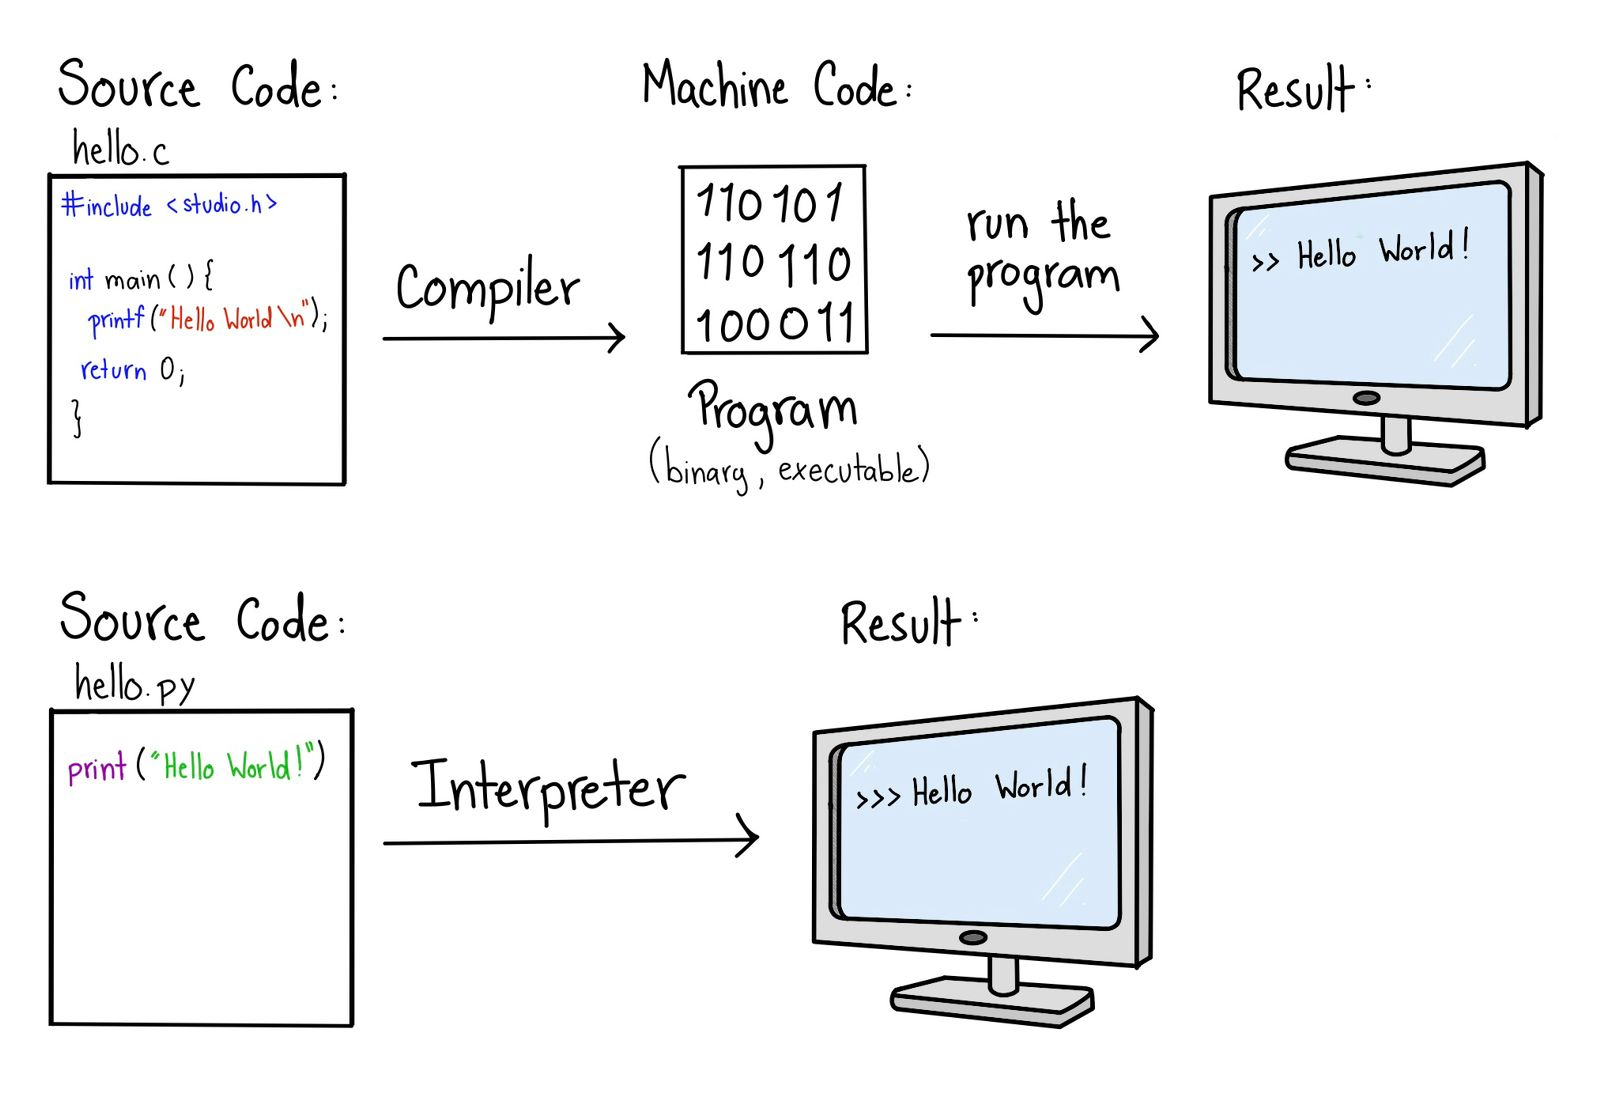
\includegraphics[width=0.75\textwidth]{fig/compiladovrsinterpretado.jpg}
    };
\end{tikzpicture}
\end{frame}

\begin{frame}[t]{C y C++}
\begin{itemize}
    \item \textbf{C} es un lenguaje de programación de propósito general, de bajo nivel, desarrollado a principios de la década de 1970 por Dennis Ritchie en los Laboratorios Bell de AT\&T. C fue creado inicialmente para desarrollar el sistema operativo Unix, y desde entonces se ha convertido en uno de los lenguajes de programación más influyentes y utilizados en la historia de la informática.
    \item \textbf{C++} es una extensión del lenguaje C, desarrollada por Bjarne Stroustrup en los años 1980. C++ se diseñó para añadir características orientadas a objetos a C, lo que lo convierte en un lenguaje híbrido que soporta tanto programación orientada a objetos como programación procedimental.
\end{itemize}
\end{frame}

\begin{frame}[t]{Variables y tipos}
\begin{itemize}
    \item \textbf{Variable} identifica una ubicación en la memoria del computador en la que puede guardar datos que pueden ser modificados durante la ejecución del programa.
    \item \textbf{Tipos de datos} define que tipo de valor y que operaciones se pueden realizar con una variable específica 
\end{itemize}
\end{frame}

\begin{frame}[t]{Tipos de datos numéricos en C y C++}
\begin{columns}[c, onlytextwidth]
    \begin{column}{0.5\textwidth}
        Tipos: 
        \begin{itemize}
            \item \textbf{int}
            \item \textbf{char}
            \item \textbf{float}
            \item \textbf{double}
            \item \textbf{void}    
        \end{itemize}
        Modificadores
        \begin{itemize}
            \item \textbf{signed}
            \item \textbf{unsigned}
            \item \textbf{short}
            \item \textbf{long}  
        \end{itemize}
    \end{column}
    \begin{column}{0.5\textwidth}
        Derivados: 
        \begin{itemize}
            \item \textbf{array}
            \item \textbf{pointer}
            \item \textbf{struct}
            \item \textbf{union}
            \item \textbf{enum}    
        \end{itemize}
        C++
        \begin{itemize}
            \item \textbf{bool}
            \item \textbf{wchar\_t}
            \item \textbf{string}
            \item \textbf{class}  
        \end{itemize}
    \end{column}
\end{columns}

\end{frame}




\begin{frame}{Ejemplo: envio de datos digitales}
Como ejemplo, vamos a simular enviar el número 221 de forma sincronica y cableada. En su versión mas básica la comunicación digital implica los siguientes pasos:
{\footnotesize
\begin{itemize}
    \item Codificación del dato: se codifica el número en formato binario, en este caso el número 221 se puede representar de forma binaria como 0b11011101
    \item Codificación de la señal: se codifica la señal de forma que un 1 corresponde a 5V y un 0 a 0V y se define el orden como MSB (most significant bit first).
    \item Sincronizar emisor y receptor: el reloj tendrá una frecuencia de 1kHz, lo que significa que se envia un bit cada 1ms.
    \item Enviar datos bit por bit: el emisor cambia el valor del bit cuando el reloj pasa de 5V a 0V y el receptor lee el bit cuando el reloj pasa de 0V a 5V
    \item Decodificar la señal: se decodifica la señal de forma que 5V corresponden a un 1 y 0V a un 0
    \item Decodificar el dato: se decodifica el número a partir del binario recibido, en este caso el binario 0b11011101 corresponde al número 221.
\end{itemize}
}
\end{frame}




\begin{frame}[t]{Señales analógicas y digitales}
Cantidad física que varia con una o mas variables independientes y que porta información relevante.\\[8pt]
Características: escalar o vectorial, discreta o continua, determinista o aleatoria.\par

\begin{tikzpicture}[remember picture, overlay]
    \node[above=0.6cm] at (current page.south) 
    {
        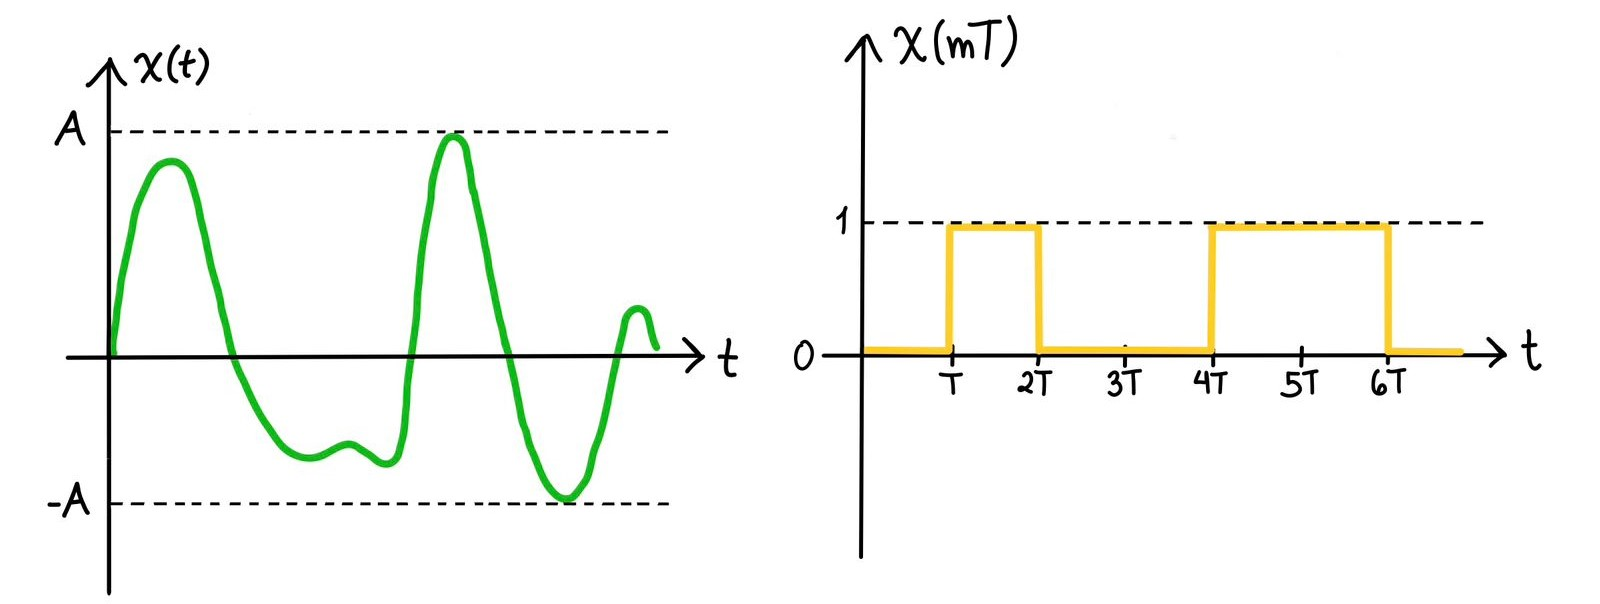
\includegraphics[width=0.8\textwidth]{fig/analogicavrsdigital.jpg}
    };
\end{tikzpicture}
\end{frame}

\begin{frame}[t]{Señales analógicas y digitales}
\textbf{Analógicas:} son señales continuas que están definidas en todos los instantes en el tiempo y tienen un infinito numero de valores posibles en cualquier intervalo.\\[8pt]
\textbf{Digitales:} Son señales discretas que tienen valores especificos en intervalos de tiempo distintos.

\begin{tikzpicture}[remember picture, overlay]
    \node[above=0.6cm] at (current page.south) 
    {
        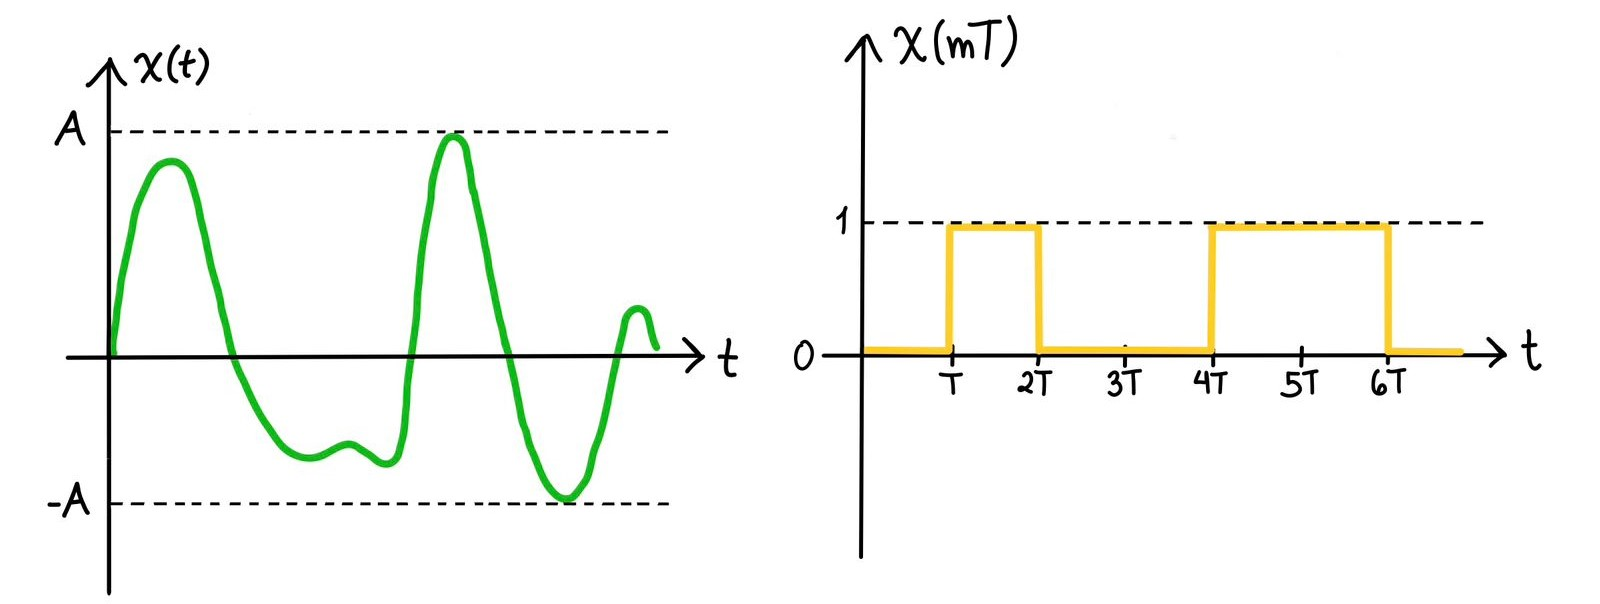
\includegraphics[width=0.8\textwidth]{fig/analogicavrsdigital.jpg}
    };
\end{tikzpicture}
\end{frame}

\begin{frame}{Sistema de adquisición de datos}
\begin{columns}[c, onlytextwidth]
    \begin{column}{0.4\textwidth}
        Un sistema de adquisición de datos es una combinación de hardware y software utilizado para recolectar, procesar y almacenar datos de mediciones de fenómenos físicos, a menudo en tiempo real.
    \end{column}
\end{columns}
\begin{tikzpicture}[remember picture, overlay]
    \node[left=-0.5cm] at (current page.east) 
    {
        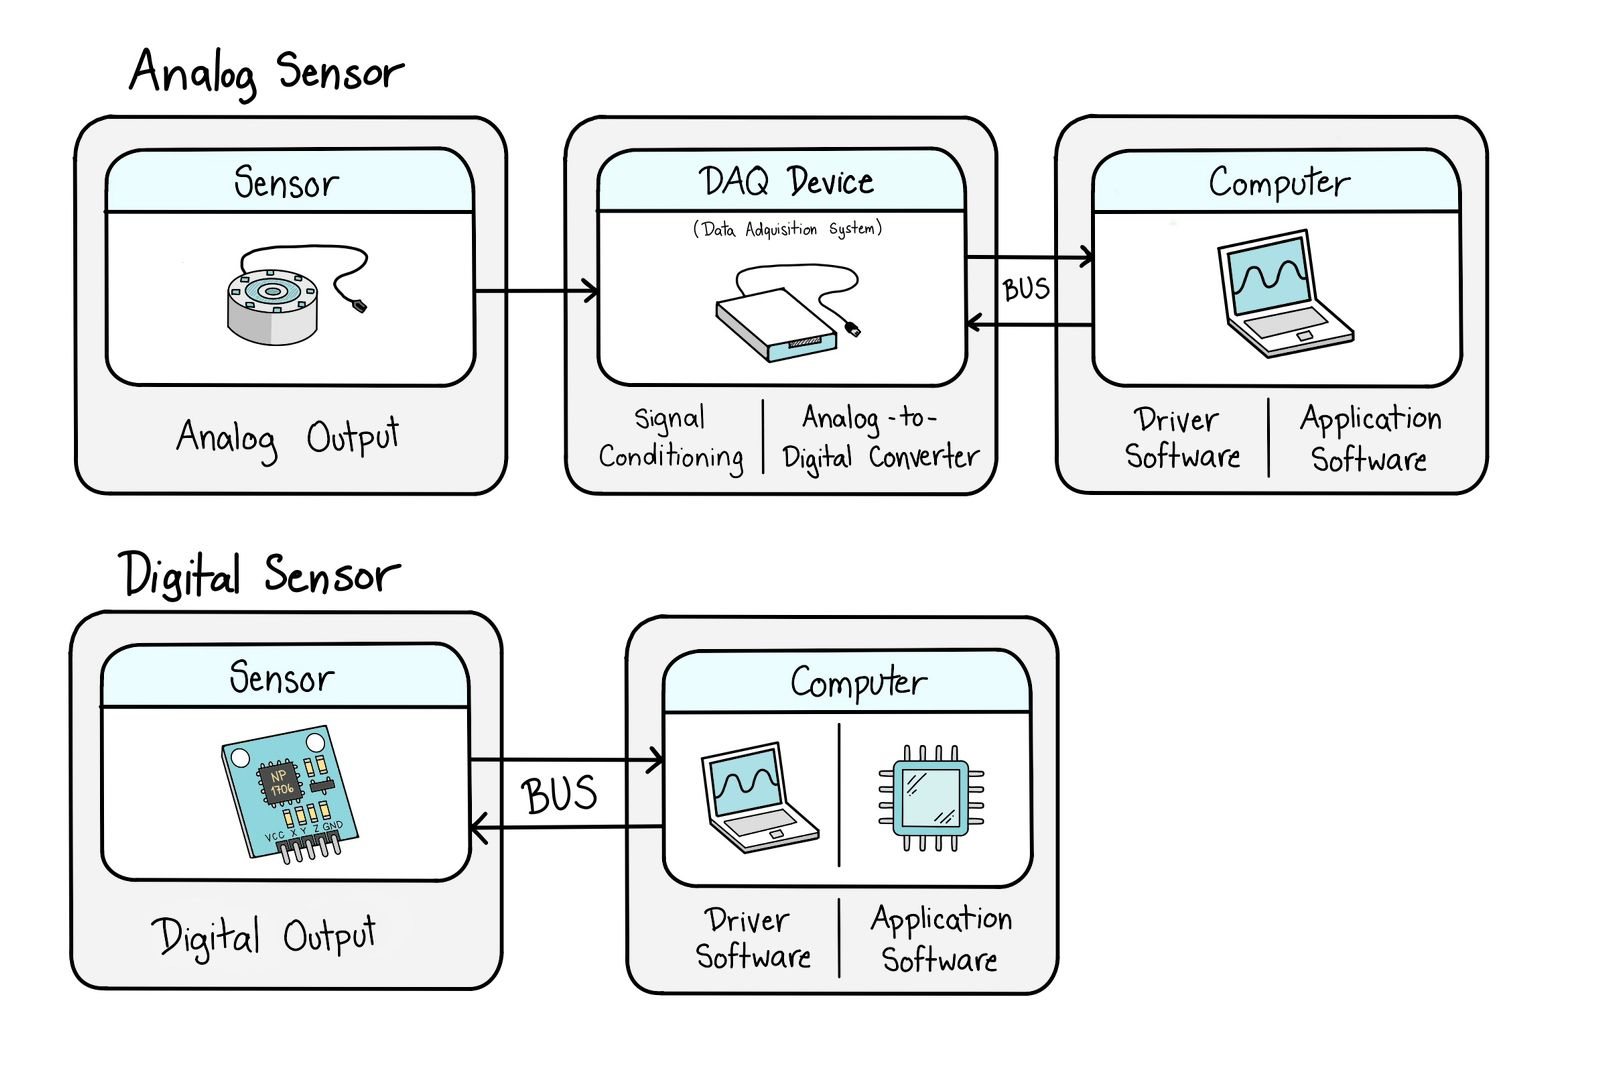
\includegraphics[width=0.7\textwidth]{fig/sistema_adquisicion.jpg}
    };
\end{tikzpicture}
\end{frame}

\begin{frame}{Acondicionamiento de señales}
Es el proceso en el que se prepara la señal para que sea adecuada para entrar en el convertidor analógico digital (ADC). Algunas de las técnicas de acondicionamiento incluyen:

\begin{itemize}
    \item Amplificación o atenuación
    \item Filtrado
    \item Aislamiento
    \item Linearización
    \item Excitación
    \item Multiplexación
\end{itemize}
\end{frame}

\begin{frame}[t]{Conversión analógica digital}
Proceso de conversión de una señal para que esta pueda ser transmitida por medios digitales
\begin{tikzpicture}[remember picture, overlay]
    \node[above=1cm] at (current page.south) 
    {
        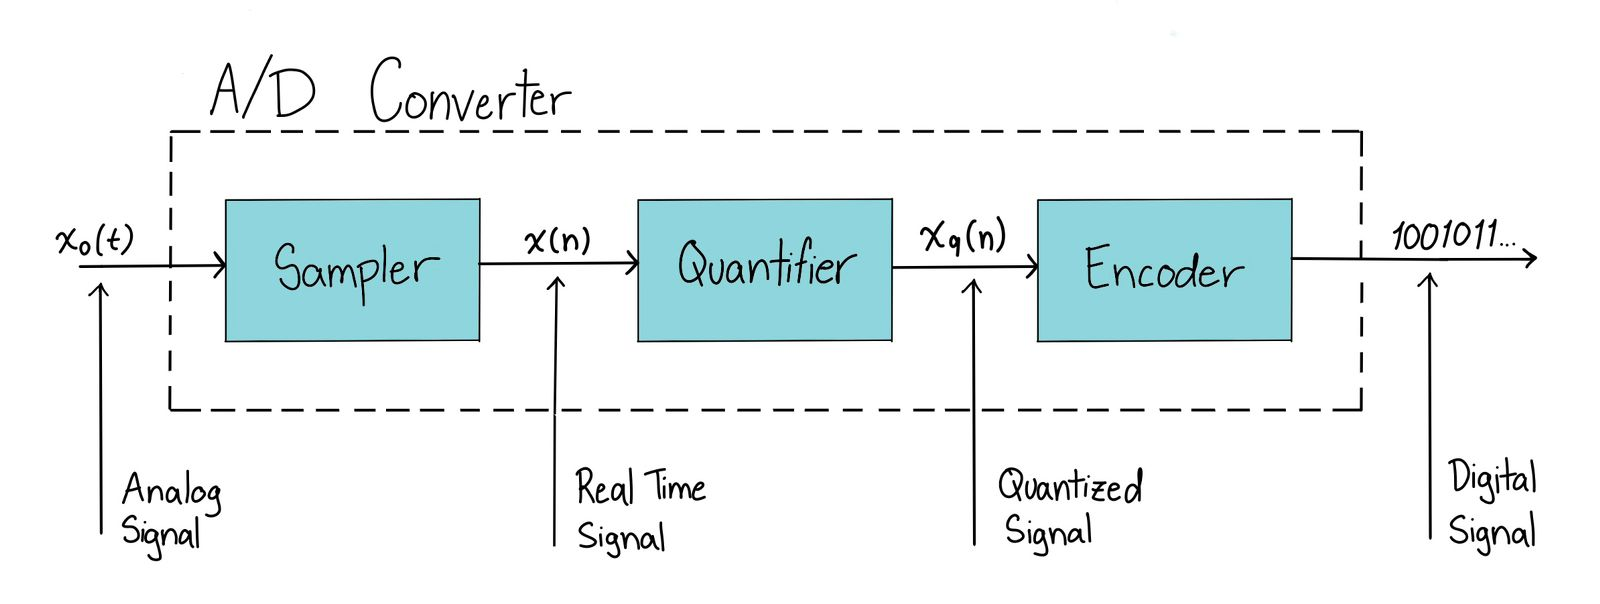
\includegraphics[width=0.8\textwidth]{fig/convAD.jpg}
    };
\end{tikzpicture}
\end{frame}

\begin{frame}[t]{Etapas de la conversión analógica digital}
\textbf{Muestreo:} se toman muestras de la señal analógica de forma periódica. Se debe respetar la frecuencia de Nyquist como mínimo: 
\begin{equation*}
    f_N=2 \cdot f_{max}
\end{equation*}

\begin{tikzpicture}[remember picture, overlay]
    \node[above=0.6cm] at (current page.south) 
    {
        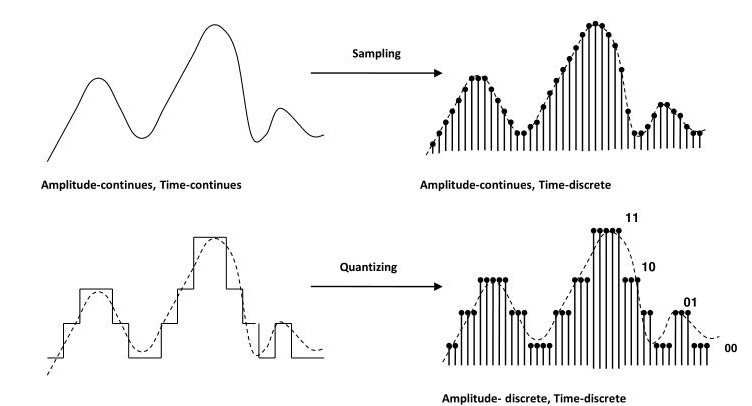
\includegraphics[width=0.8\textwidth]{fig/muestreo.jpg}
    };
\end{tikzpicture}
\end{frame}

\begin{frame}[t]{Etapas de la conversión analógica digital}
\textbf{Cuantización:} se asigna el nivel al que cada muestra pertenece

\begin{align*}
\mathrm{Resolución}\hspace{0.5cm}\Delta=\dfrac{\mathbf{Rango}}{2^{b}-1} \hspace{0.8cm} \mathrm{Error\,de\,cuantización}\hspace{0.5cm}|e_{q}| \leq \dfrac{\Delta}{2}
\end{align*}

\begin{tikzpicture}[remember picture, overlay]
    \node[above=0.6cm] at (current page.south) 
    {
        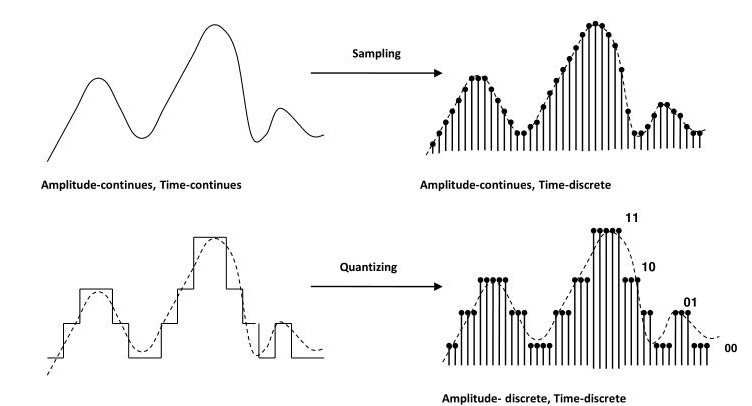
\includegraphics[width=0.8\textwidth]{fig/muestreo.jpg}
    };
\end{tikzpicture}
\end{frame}


\begin{frame}[t]{Etapas de la conversión analógica digital}
\textbf{Codificación:} se codifica cada muestra de acuerdo al nivel

\begin{tikzpicture}[remember picture, overlay]
    \node[above=0.6cm] at (current page.south) 
    {
        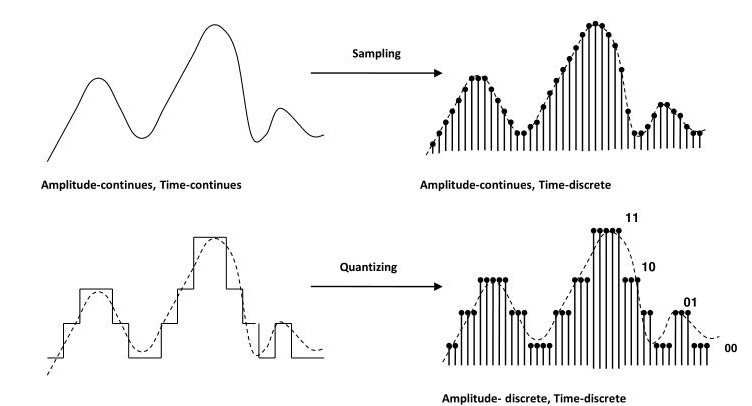
\includegraphics[width=0.8\textwidth]{fig/muestreo.jpg}
    };
\end{tikzpicture}
\end{frame}



% \begin{frame}{Señales de entrada y salida}
%     \begin{columns}[c, onlytextwidth]
%         \begin{column}{0.4\textwidth}
%              \begin{itemize}
%                 \item Entradas: son las variables que afectan el comportamiento del sistema
%                 \item Salidas: son las variables que son definidas por el sistema
%              \end{itemize}
%         \end{column}
%         \begin{column}{0.6\textwidth}
%             \begin{center}
%                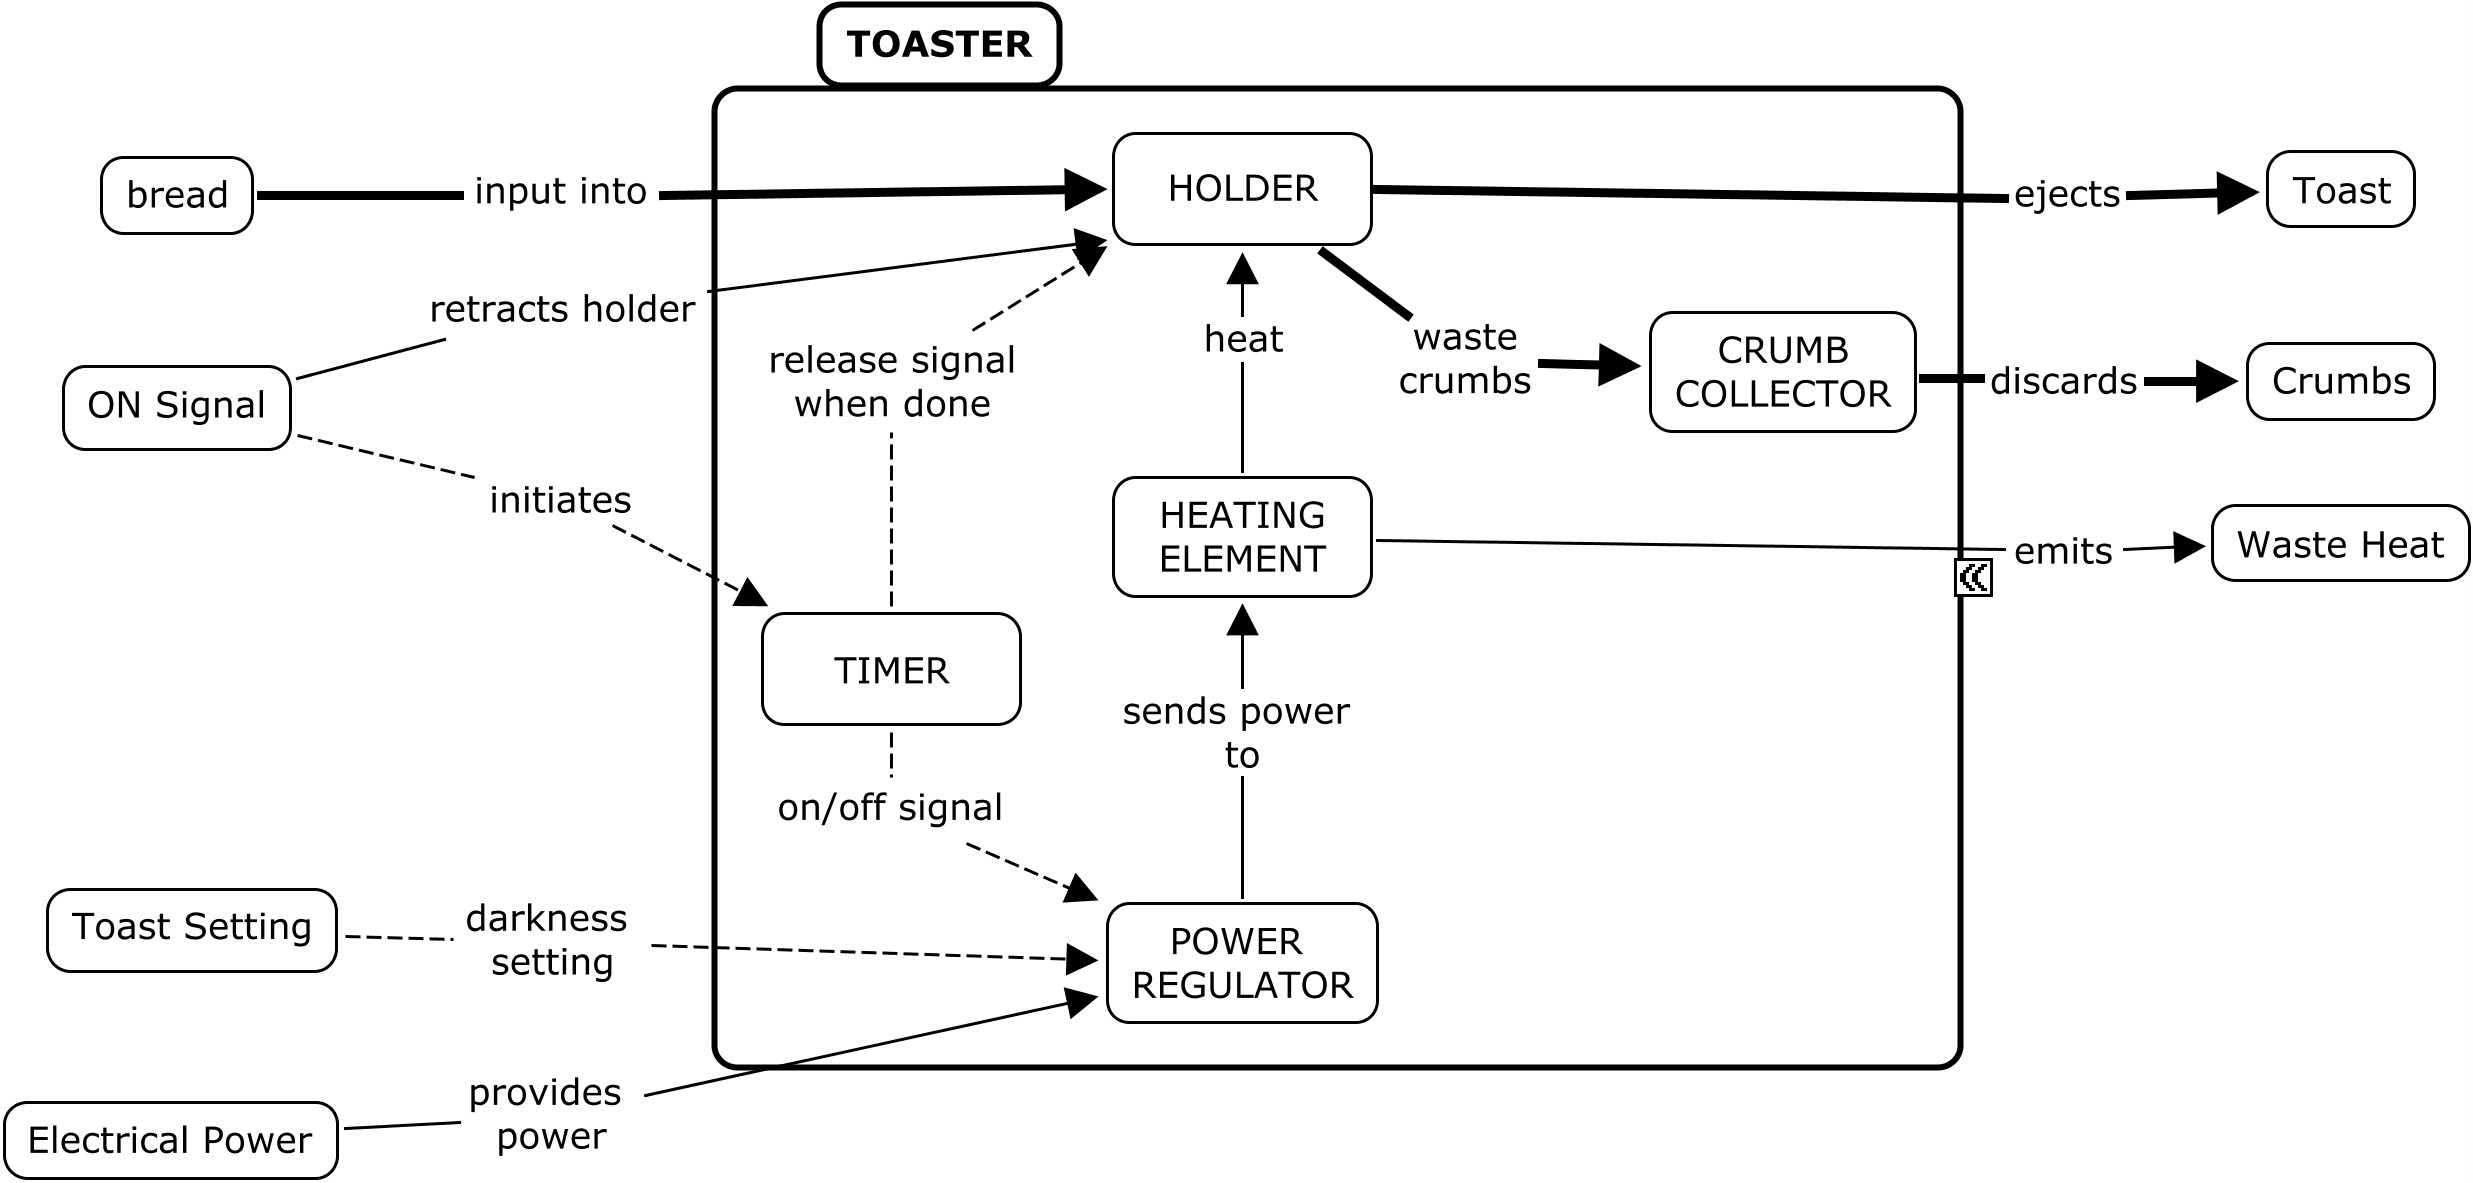
\includegraphics[width=\textwidth]{fig/tostadora.jpg}\\
%                \tiny{Tomado de \href{https://deseng.ryerson.ca/dokuwiki/_detail/design:toasterarchitecture.jpg?id=design\%3Asystem_diagram}{aquí}}
%             \end{center}
%         \end{column}
%     \end{columns}
% \end{frame}

% \begin{frame}{Modelos}
%     \begin{columns}[c, onlytextwidth]
%         \begin{column}{0.5\textwidth}
%         Un modelo es una abstracción matemática de un sistema.\\[8pt]
%         \begin{itemize}
%             \item Se modela el sistema en base a ecuaciones
%             \item Es una simplificación del sistema real
%             \item Solo es valido en ciertas condiciones y/o rangos
%         \end{itemize}
%         \end{column}
%         \begin{column}{0.5\textwidth}
%             \begin{center}
%                 \begin{circuitikz}
%                     \draw 
%                     (0,0)
%                         to[cV, l=$OCV(z)$]
%                     (0,3)
%                         to[R, l=$R_0$,i=$i(t)$,-o]
%                     (3,3)
%                         to[open,v^=$v(t)$]
%                     (3,0)
%                         to[short,o-]
%                     (0,0)
%                     ;
%                 \end{circuitikz}\\[8pt]
%                 \footnotesize{Modelo Rint de una celda electroquímica}
%             \end{center}
%         \end{column}
%     \end{columns}
% \end{frame}

% \begin{frame}{Transductores, sensores y actuadores}
%     \begin{columns}[c, onlytextwidth]
%         \begin{column}{0.6\textwidth}
%         Para los efectos de este curso...\\[8pt]
%         \begin{itemize}
%             \item \textbf{Transductor:} dispositivo que convierte una señal de un tipo de energía a una señal correspondiente pero con un tipo de energía diferente.
%             \item \textbf{Sensor:} transductor que convierte una señal física a un señal eléctrica
%             \item \textbf{Actuador:} transductor que convierte una señal eléctrica a un señal física
%         \end{itemize}
%         \end{column}
%         \begin{column}{0.4\textwidth}
%             \begin{center}
%                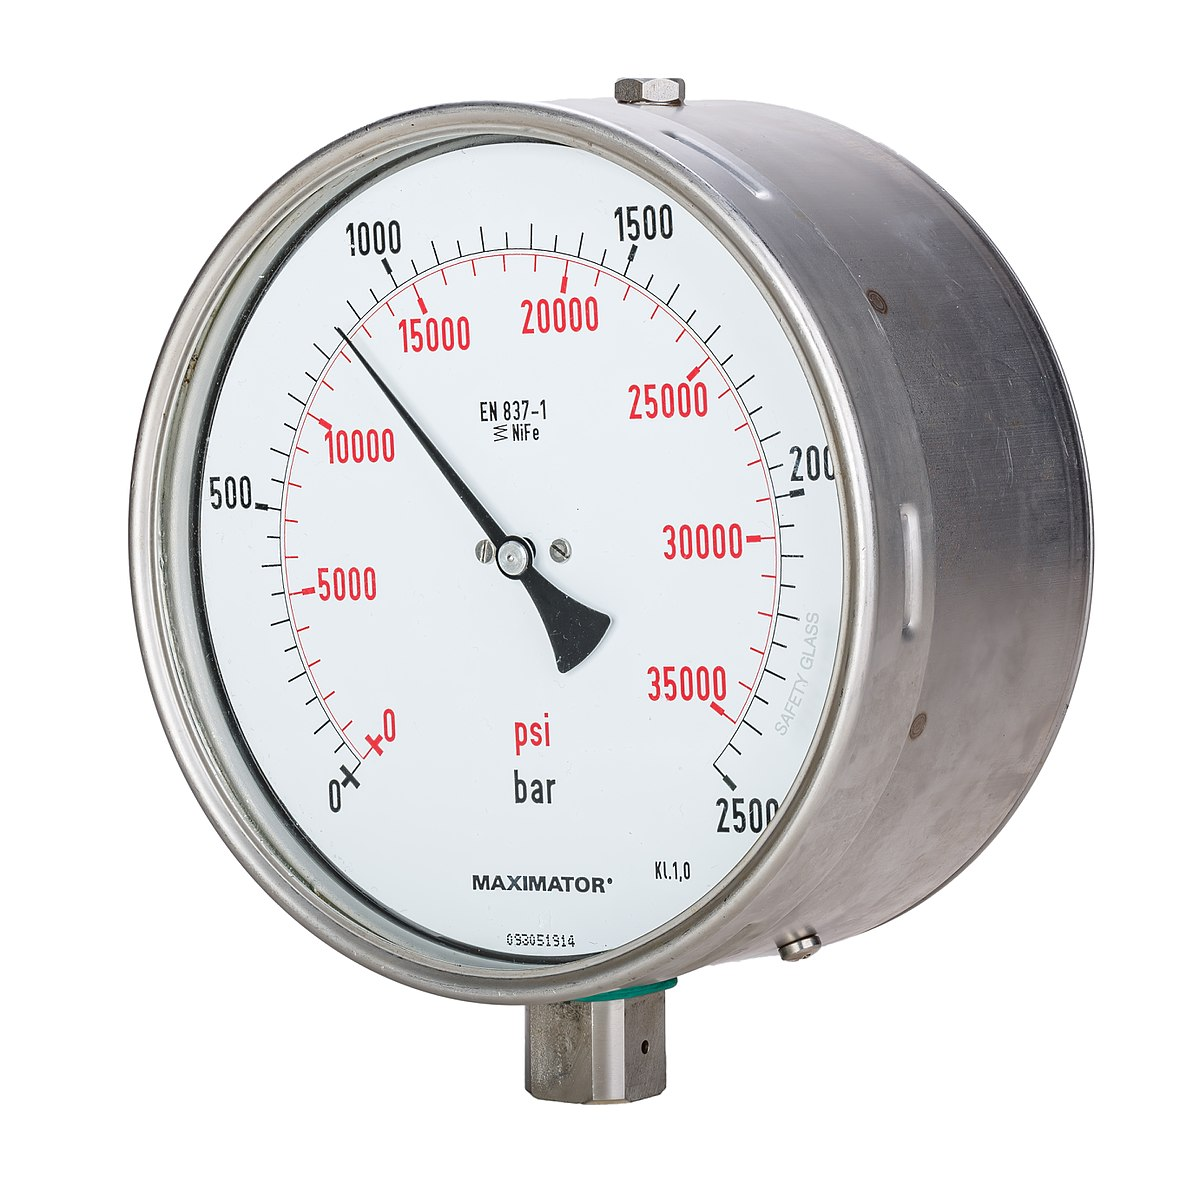
\includegraphics[width=0.8\textwidth]{fig/bourdon.jpg}\\
%                \tiny{Tomado de \href{https://upload.wikimedia.org/wikipedia/commons/thumb/7/74/MAXIMATOR-High-Pressure-Manometer-01a.jpg/1200px-MAXIMATOR-High-Pressure-Manometer-01a.jpg}{aquí}}
%             \end{center}
%         \end{column}
%     \end{columns}
% \end{frame}

% \begin{frame}{Sensores directos y complejos}
%     \begin{columns}[c, onlytextwidth]
%         \begin{column}{0.5\textwidth}
%         Sensor directo
%             \begin{tikzpicture}
%                 \node[draw,minimum width=2cm,minimum height=1.2cm](sensor) {sensor};
%                 \draw[>=latex, thick, ->](sensor) --++ (-3,0) -- (sensor);
%                 \node[left=1,above] at (sensor.west){\small estímulo};
%                 \draw[>=latex, thick, ->](sensor) -- (sensor) --++ (3,0);
%                 \node[right=1,above] at (sensor.east){\small señal};
%                 \node[right=1,below] at (sensor.east){\small eléctrica};
%                 \draw[\blackandwhite] (-3,-1.5) rectangle (3,3);
%             \end{tikzpicture}
%         \end{column}
%         \begin{column}{0.5\textwidth}
%         Sensor complejo
%             \begin{tikzpicture}
%             \node[draw,minimum width=1cm,minimum height=1cm](s1) {trans};
%             \draw[>=latex, thick, ->](s1) --++ (-2,0) -- (s1);
%             \node[left=0.75,above] at (s1.west){\small estímulo};
%             \node[draw,minimum width=1cm,minimum height=1cm,right of=s1,node distance=2cm](s2) {sens};
%             \draw[>=latex, thick, ->](s2) -- (s2) --++ (2,0);
%             \node[right=0.75,above] at (s2.east){\small señal};
%             \node[right=0.75,below] at (s2.east){\small eléctrica};
%             \draw[>=latex, thick, ->](s1) -- (s2);
%             \draw[\blackandwhite] (-2,-1.5) rectangle (4,3);
%             \draw[black, dashed] (0.75,-1) rectangle (4,1.5)node[midway,above=0.7]{\small sensor directo};
%             \end{tikzpicture}
%         \end{column}
%     \end{columns}
% \end{frame}

% \begin{frame}{Sensores pasivos y activos}
%     \begin{columns}[c, onlytextwidth]
%         \begin{column}{0.5\textwidth}
%         Sensor pasivo
%             \begin{tikzpicture}
%                 \node[draw,minimum width=2cm,minimum height=1.2cm](sensor) {sensor};
%                 \draw[>=latex, thick, ->](sensor) --++ (-3,0) -- (sensor);
%                 \node[left=1,above] at (sensor.west){\small estímulo};
%                 \draw[>=latex, thick, ->](sensor) -- (sensor) --++ (3,0);
%                 \node[right=1,above] at (sensor.east){\small señal};
%                 \node[right=1,below] at (sensor.east){\small eléctrica};
%                 \draw[\blackandwhite] (-3,-1.5) rectangle (3,3);
%             \end{tikzpicture}
%         \end{column}
%         \begin{column}{0.5\textwidth}
%         Sensor activo
%             \begin{tikzpicture}
%                 \node[draw,minimum width=2cm,minimum height=1.2cm](sensor) {sensor};
%                 \draw[>=latex, thick, ->](sensor) --++ (-3,0) -- (sensor);
%                 \node[left=1,above] at (sensor.west){\small estímulo};
%                 \draw[>=latex, thick, ->](sensor) -- (sensor) --++ (3,0);
%                 \node[right=1,above] at (sensor.east){\small señal};
%                 \node[right=1,below] at (sensor.east){\small eléctrica};
%                 \draw[>=latex, thick, ->](sensor) --++ (0,+2) -- (sensor);
%                 \node[above=1.5] at (sensor.north){\small excitación};
%                 \draw[\blackandwhite] (-3,-1.5) rectangle (3,3);
%             \end{tikzpicture}
%         \end{column}
%     \end{columns}
% \end{frame}

% \begin{frame}{Referencias}

% \bibliographystyle{ieeetr}
% \footnotesize
% \bibliography{comunes/referencias}

% \end{frame}

\end{document}